\documentclass[article,a4paper]{IEEEtran}
\usepackage{lipsum}
\usepackage[backend=biber]{biblatex}
\usepackage{graphicx}

\addbibresource{refs.bib}
\title{Building Smarter Homestead with IoT: Harnessing MQTT, Zigbee, and LoRaWAN}
\author{
\IEEEauthorblockN{Anton Odén}\\
\IEEEauthorblockA{Dept. of Maths and Computer Science\\Karlstad University\\
651 88 KARLSTAD, Sweden}\\
anton.oden@outlook.com
}

\begin{document}

\maketitle

    \begin{abstract}
        This article examines IoT wireless communication protocols—LoRaWAN, Zigbee, and MQTT. It explores frequency band management, energy-efficient mesh networking, and lightweight messaging. By analyzing technical principles and regulatory constraints, the piece uncovers how these protocols collaboratively empower applications from smart homes to expansive sensor networks, driving modern connectivity forward.    
    \end{abstract}

    \section{Introduction}
    In today's hyper-connected era, the Internet of Things is no longer a futuristic concept. As our environment becomes cluttered by smart devices and sensor networks the challenge becomes how can we orchestrate a symphony of machines to talk to each other efficiently, reliably, and within stringent power budgets? This article dives into three vital protocol and heroes in the IoT revolution: LoRaWAN, Zigbee and MQTT. 
    \newline\newline
    We begin by exploring wireless communication in it's form as radio waves and the strategic allocation of frequency bands as those as everything else has limitatons. Zigbee, with it's implementation of a mesh network and LoRaWAN's long-range capabilities and ingenious use of Chirp Spread Spectrum technology. Meanwhile, MQTT stands out as a lightweight messaging protocol that elegantly manages data flow, ensuring that every byte is efficiently delivered across the network. The article is more reliant on the background and leaves proposed future endevours for the writer and reader to look into. 
    \section{Background}
    Communication in IoT is dependent on wireless communication, cause to connect all things by wire would quickly cover much of our space with wires and our wire-bill would match if not superseed the remaining infrastructure. Wireless communicaion could better be described as radio signals. Radio signals can be modulated to communicate at frequency, amplitud and phase and to avoid collision between different radio signals rules has been applied to what application could use what frequency. As radiosignals is used for defence capabilities there are hefty punishment \cite{RFlaw} for transmitting in frequensies not sactioned by regional authority. Thought these rules could vary globally the ISM-bands different frequencies does has a globally ok coverage making it easier to produce communication hardware. For commercial usage different parts of the ISM-band has been opened/allowed to be used \cite{ISM-band1} and the most common commercial standard today in homes, offices, cafés etc. is IEEE 802.11, containing the commonly known WiFi protocol. Communicating at 2400-2483MHz (ISM-band), 5150-5350MHz, 5470-5725 (RLAN, EU standard EN 301 893) and newly introduced 5945-6425MHz (RLAN, EU standard EN 303 687) in WiFi 7 within Europe. \cite{ISM-bandEUR}. Starting from 2.4GHz in 1997 different frequencies bands has been added to satisfy our "desperate" need to high resolution video streaming. 
    \newline\newline
    One problem for IoT end devices that could be running on battery is that WiFi in its aim to give the user high data rate (bandwidth) is power consuming. WiFi is designed for high bandwidth that results in higher power consumption and for this reasons, new standards has been introduced to IEEE 802 family. 
    \newline\newline
    IEEE 802.15.4, which goes under the name Low-Rate Wireless Personal Area Network (LR-WPAN) is written with low power consumption in mind. The standard is grandfather of protocols such as Zigbee, 6LoWPAN, Thread, SNAP etc. Zigbee was first drafted 2004 and has became famous for usage in smart home implementations. It communicates at the 2400-2483MHz, which is same as WiFi. Also 868-868MHz in Europe and 902-928MHz in North America. Why the split between europe and north america may be Europe having more military applications communicating on 902-928MHz bandwidth \cite{ISM-bandEUR}. Getting the extra communication spectrums makes it easier for the protocol to communicate in highly density Wifi areas. 
    \begin{figure}
        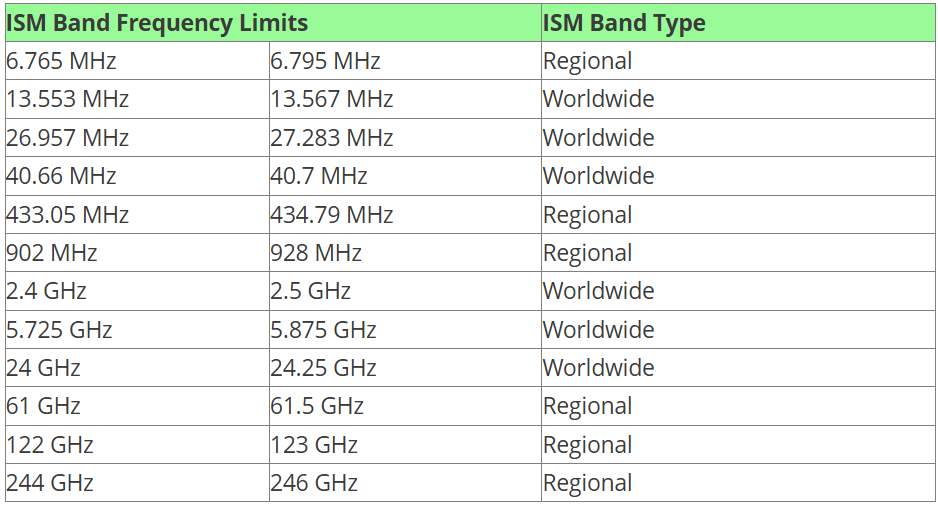
\includegraphics[width=\columnwidth]{ISM-band.png} 
        \caption{ISM-band frequency limits from \cite{ISM-band1}}
        \label{fig1:ISM-band frequency limits}   
    \end{figure}
    \ref{fig1:ISM-band frequency limits}
    Units within a zigbee network are categoriesed into three types. Coordinator, routers and end devices. The routers could be and often are an end device at the same time. The routers extend the physical range of the network and makes the network reliability as if one router goes offline the network so communication is not broken. This presupposes that end devices has more than one router in reachable range that can reach other parts of the network. The term mesh network is coined describing a zigbee network thought the network could also be structured in a star or tree topology also. "Mesh network: This is a network in which the routing of messages is performed as a decentrilized, cooperative proces involving many peer devices routing on each other's behalf." \cite{ZigbeeSpec}. So the routing devices are enabler of mesh network. The coordinator is only one within the personal area network and it is responsible of adding and decoupling devices to the network and the coordinator must be a fully functional device. End devices are all the things we want to connect in our IoT, usually a sensor/measuring instrument or some kind of actuator. 
    \newline\newline
    Another protocol in the LR-WPAN family is LoRaWAN which stand for Long Range Wide Area Network. It was developed for longer range communication. First of LoRa was developed for radiofrequency of 2-10km and then LoRaWAN was added on top to add network layer capabilities to the physical communication. LoRa radio frequency is divided between regions. Europe communicates 863-870MHz, USA 902-928MHz, China 470-510 and 779-787MHz etc. The division in the worlds LoRaWAN communication is illustraded in the fig3.
    \begin{figure}
        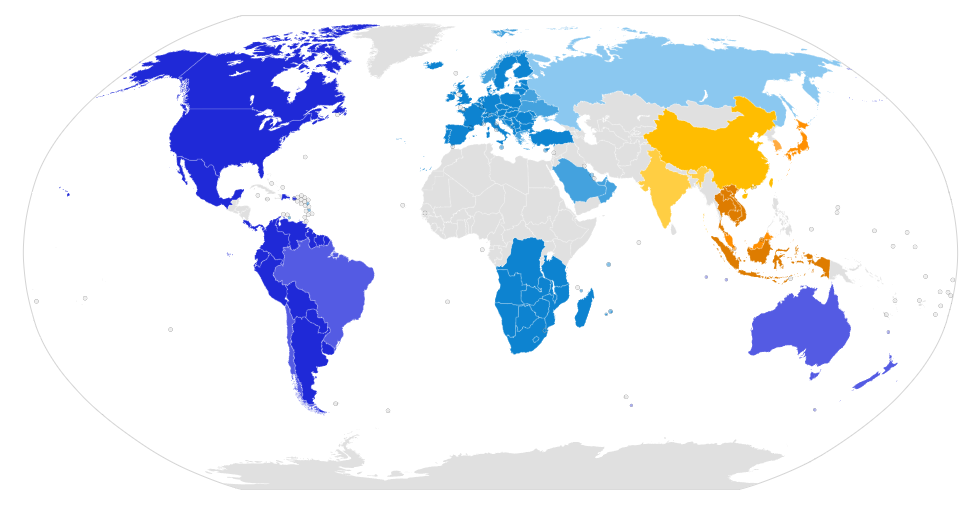
\includegraphics[width=\columnwidth]{LoRaWANdivide.png} 
        \caption{Map showing different frequencies in LoRa from \cite{LoRaWanfreqCountry}}
        \label{fig3:freq LoRaWAN}   
    \end{figure}
    \ref{fig3:freq LoRaWAN}
    LoRa transmit data with an technique called Chirp Spread Spectrum (CSS) that means that the transmitting is constantly modulates frequency \cite{LoraWanSpecOverview,LoRaTutorial}. For example Europes designated LoRa bandwidth 863-870MHz is further divided into allowed tranmission channels (regional channel plan) for uplink and downlink. One of those uplinks channels are 125kHz around 868,3MHz. Within that channel a transmission of bits is done by constantly modulating the frequency from lowest point 868,225MHz to channels highest point 868,375MHz (Eg. One chirp). Depending on what starting point within the chirp a specific symbol is being transmitted. A new tranmission allways starts with a set number of upchirps followed by some downchirps, letting the reciever know a datatransmission is starting. Transmission shifts between the allowed transmissionchannels in a pseudo-radom fashion. These frequency modulation and transmission shifting makes LoRa very resiliant to other transmission within the same bandwidth as the reciever can ignore other senders signals at noise as their current chirp status is with low propability the same and as LoRa is having a very far range capabilites alot of noise will be present.      
    \newline\newline
    To add functionality to the network another protocol is needed on top of network protocols, for example Zigbee or LoRaWAN that is used for the communication. The most famous protocol for this is Message Queue Telemetry Transport (MQTT) \cite{mqtt3.1.1,mqtt5.0}. MQTT filters all messages in a publish/subscribe manor. So MQTT terminology divide the network up in MQTT server/broker and MQTT clients, where the MQTT server is the central hub in the messaging system. All clients connected to the server published messages to the server, all published messages are labeled with a topic (usally friendly devicename for sensor IoT devices). All clients in the MQTT network can subscribe to specified published topics. So for example if an IRsensor send/publish a message with topic "AwesomeRobotSolutionIRSensor", all clients that are subscribing to topic "AwesomeRobotSolutionIRSensor" will recieve the published message via the MQTT broker. The MQTT header is designed to be lightweight which is convinient for IoT devices with low power consumption. The most basic ping message is reduced to only 2 bytes. To compare ICMP (Internet Control Message Protocol) requeries 8bytes header + 20 bytes IP header for a ping request \cite{ICMPping}. MQTT with it's 2bytes + zigbee network header of 8 bytes is 18 bytes or 2.8 times less in size. These reduction in packet sizes of the IoT protocols is what makes the low power consumption possible.
    \newline\newline
    A feature in MQTT is Quality of Service (QoS). In MQTT is is divided into 3 different cases \cite{mqtt3.1.1,mqtt5.0}. Both subsribing and publishing links does has the QoS setting to them. It is up to the user to set how important the messages sent are. Overhead (power consumption) is raised with higher level quality of service:
    \begin{itemize}
        \item QoS 0: At most once delivery. Messages are published with no demand of acknowledge if they got to the reciever end. -> PUBLISH
        \item QoS 1: At least once delivery. Reciever ackknowledge recieved message to sender making sender dicard sent message from memory buffer. If now ackknowledge recieved by sender a the message is published again until an ackknowledge is recieved. Hence final reciever could recieve multiple publishing messages of same type. -> PUBLISH <- PUBACK (fig2)
        \item QoS 2: Exactly once delivery. Adds a second back and forward between reciever and sender so that reciever does not register and forward multiple messages of the same publishing source. -> PUBLISH <- PUBREC -> PUBREL <- PUBCOMP.  
    \end{itemize}
    \begin{figure}
        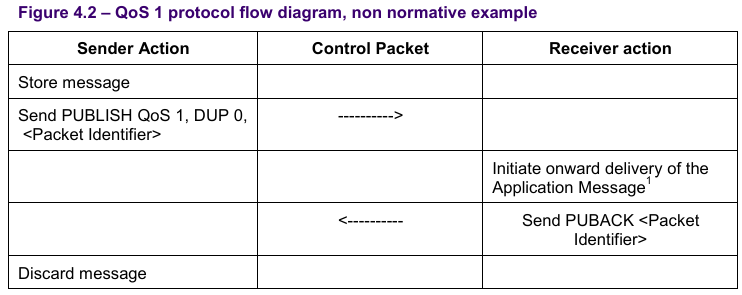
\includegraphics[width=\columnwidth]{QoS1.png} 
        \caption{QoS flow diagram from \cite{mqtt3.1.1}}
        \label{fig2:QoS1 flow diagram}   
    \end{figure}
    \ref{fig2:QoS1 flow diagram} 
    
    Topics in MQTT \cite{mqtt3.1.1} is structured with forward slashes to divide topics in a hierarchy with levels similar to folders and files in a file system.
    \begin{itemize}
        \item home/livingroom/temphum
        \item home/livingroom/lamp
    \end{itemize} 
    Knowing this a client can subscribe to all sensortypes with a single topic subscription using wildcards which could be stated to ignore different levels in the topic hierarchy. For example we can subsribe to all topics within our livingroom by subsribing to home/livingroom/\#. Or if we have lamps in other rooms in our home we could subsribe to home/+/lamp. As example shows we have + and \# sign to work with when using wildcards. There are more to talk about regarding MQTT but to finish with it is important to know that it's currently two versions of MQTT thats active today. MQTT 3.1.1 released in 2014 and MQTT 5.0 released in 2019. There a many examples on different protocols with MQTT alike features like MQTT-SN, ZeroMQ and AMQP that are worth mentioning thought MQTT is becoming industry standard. Some popular brokers/serversoftware using the MQTT protocol is Mosquitto, EMQX, VerneMQ, NanoMQ \cite{PopularMQTTprotocol}  There are also competing protocols to MQTT even if MQTT is becoming/already become industry standard.

    \section{A Challenge of Smart Home Networking}
    We have now went throught three different protocols. Two for communication (LoRaWAN and Zigbee) and another layor on top to be able to decide which device to transmitt to (MQTT). These are only a few of many different protocols and a challenge is to decide what protocol to use. Wifi has became synonymys with internet communication but as it's energy consumption is not suitable for battery powered units another protocol is needed, LP-WAN protocols are a good direction to look at. One problem is that alot of different protocols are competeing in trying to be the protocol for smart home sensors. The lower range for for example in Zigbee is dependent on mesh network with powerplugdriven router devices to get reception in the home as a whole. Soyou get locked in to one communication protocol that may be good for one thing but lack in others. Critics against Zigbee for example is the lack of IP-adressing and security. One movement to combine all protocols is in a overheadprotocol called Matter \cite{Matterspec} that is overseen by Connectivity Standards Alliance (former Zigbee Alliance). The specification is relative new with first revision released 2020 and its main selling points is added IP-adresses and security. The alliance is a joint effort from over 500 companies containing containing alot of big players sush as Amazon, IKEA, Google, Apple, Schneider etc. Matter could become one among many standards, enhancing the problem with "to many standards to choose from". Where inoperability among smart units in homes is present, but Matter is atleast an effort to make bridges.  
    \begin{figure}
        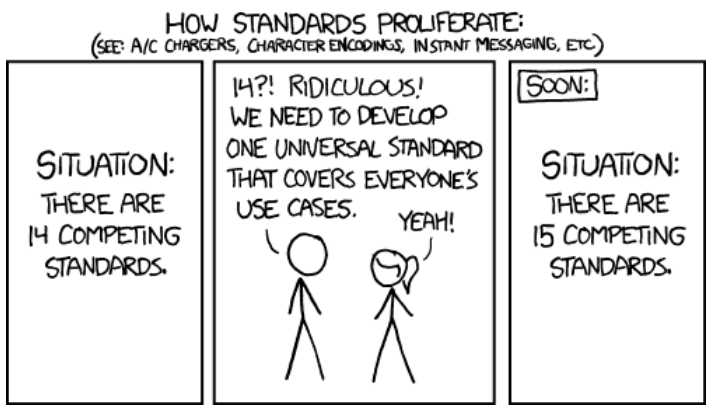
\includegraphics[width=\columnwidth]{NewStandard.png} 
        \caption{ fig4: Standards (xkcd -https://xkcd.com/927/). Licensed under CC BY-NC 2.5 License (https: //creativecommons.org/licenses/by-nc/2.5/) }
        \label{fig4: Standards (xkcd -https://xkcd.com/927/). Licensed under CC BY-NC 2.5 License (https: //creativecommons.org/licenses/by-nc/2.5/)}   
    \end{figure}
    \ref{fig4: Standards (xkcd -https://xkcd.com/927/). Licensed under CC BY-NC 2.5 License (https: //creativecommons.org/licenses/by-nc/2.5/)} 
    \section{Why Combine MQTT, Zigbee, and LoRaWan?}
    In a countryside home the area to cover often is bigger than in a a single house in the city. Alot of buildings outside and earthcellars for example could need more range capabilities that LoRaWAN can offer contra Zigbee. Also the buildings may lack electricity than further makes it harder to get in range with Zigbee as no routing devices can be added to the buildings. A homestead could have acres of land to collect data from where Zigbee lacks the necessary length. It adds complexity to the home network in that a second controller is needed for LoRaWAN units but as the alternative would be to bring electricity to the locations in need of datacollection in may be cheaper. Then if the initial cost of also setting up an LoRaWAN network has passed the home has the flexibility in place of choosing between two networks besides Wifi. Zigbee for low power short range, LoRaWAN for low power long range and Wifi for great bandwidth and lets say medium range even if it's closer to Zigbees short range. 
    \section{LoRaWAN Device Classes}
    LoraWAN devices is has the availability to be three different classes that decided how much the devices is going to listen för transmissions. \textbf{Class A} is eventdriven based on the end device communication to the network. When an end device is finish transmitting data it listen for a respons from the network. If no response was given the device goes into sleep mode for a while and then listens again for a moment. If no respons was recieved the second time the end device goes into sleep until next time it wants to transmitt. The timing of the period that the end device is awake listening to transmission can be configured and the network knows about the end device configuration. Second \textbf{Class B} named Beacon has the same settings as class A but adding on top of that the devices listens after transmissions in a fixed timely fashion adding the complexity to the network that the end devices internal clocks needs to be syncronised with the network. Third \textbf{Class C} is allways listeing to transmission when it's not transmitting. 
    \section{Designing the Network Architecture}
    So in a LoRaWAN network we got the end devices. We also got something called gateway devices that is the bridge between network server and the end devices. Same as in a Zigbee network these serves as the extender of the network. When LoRaWAN network server then wants to communicate back it does is via the gateway with the higest Received Signal Strength Indicator (RSSI) that is a value that the gateways adds to the transmission that is forwared to the network servers. This means that the network servers is handed multiple packets from the same end device transmission and it is the network server that sorts out the duplication. The network servers the forward messages to the application servers that contain for example MQTT that bring smartness to the network. The application servers also has a join server that is initializing the end devices in the network. The join server in communication with end device sets up 128-bit AES encryption for both the network communication, that the gateways and network servers can decrypt and application communication that only the application server can decrypt. This ensures that only the application and end devices can read the data being transmitted and the network transmission makes sure only the private network can read the messages being sent. As communication being done in long range (2-10km) eavesdropping would be to easy be gona unnoticed otherwise. 
    \begin{figure}
        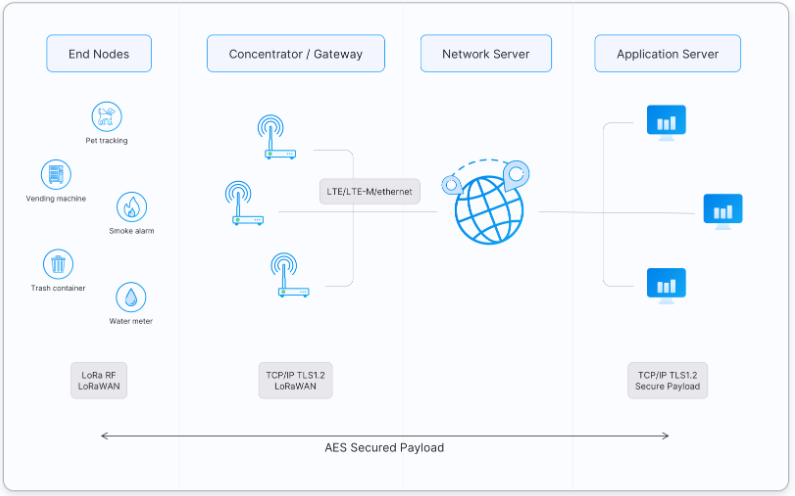
\includegraphics[width=\columnwidth]{LoRaWANnetwork.png} 
        \caption{ fig5: LoRaWAN network architecture from \cite{LoRaWANarchi} }
        \label{fig5:LoRaWAN network architecture }   
    \end{figure}
    \ref{fig5:LoRaWAN network architecture} 
    \newline\newline
    Both Zigbee and LoRaWAN is dependent on having one network server orchestrating the network. This is one critic againts the protocols as the network server becomes a single point of failure. Failures in gateways and routers is thought mitigated by both networks architecture as long as every end node has more than one gateway/router within reach.    
    \section{Practical Use Cases}
    One way to combine LoRaWANs long range and Zigbees cheep producs I stumbled upon is LoRa Databridge \cite{LoRabridge}. Developed during 2021 it creates two gateways that communicate with eachother. Something that could mitigate having a building further away from over mainhouse mesh zigbee network. Then LoRa Databridge could forward data collection points to our main network. The project look promising for homestead implementation and others ofc. Having concrete walls and floors Zigbee does have problems communicating down to the basement. Implementing a couple of LoRaBridges could mitigate those problems. 
    \begin{figure}
        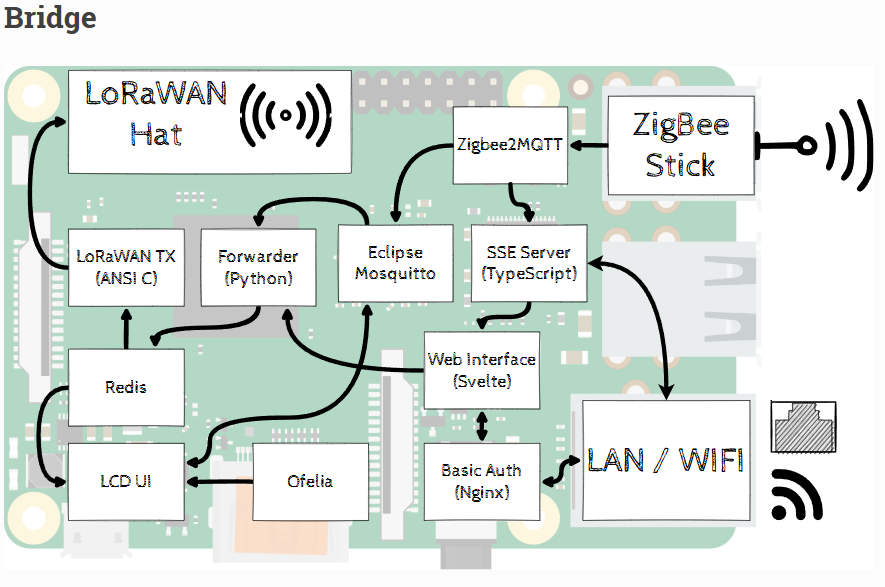
\includegraphics[width=\columnwidth]{LoRaBridge.png} 
        \caption{ fig6: LoRabridge software \cite{LoRaBridgeDocs} }
        \label{fig6: LoRabridge software }   
    \end{figure}
    \ref{fig6: LoRabridge software} 
    Another podcast having a disussion \cite{LoRaWANpodcast} with Wienke Giezeman from The Things Industries disuss LoRaWAN great potential to monitor waterpipes. They discuss that bigger enterprises having hundred of thosand nodes for water monitoring may be designing there own communication protocol but for smaller scale (or normal scale) LoRaWAN comes in handy being an open protocol for usage there is off the shelf hardware that is possible for local smaller municipality or in my case a local joint waterassosication between 50 neighbours could install. I'm looking forward to investigating what possibities exists for this. 
    \section{Future Trends and Innovations}
    As prior discussed Matter is a joint endovour were only time will tell if it becomes an industry standard. The blogposts read does give some insites into some of the big companies (Apple, Amazon etc) does not release all their new devices being Matter compatible \cite{BlogMatter}. So I belive we will still need to invest in gateways infrastructure inmultiple communication protocols in our smart homes. Even Matter that is suppose to unite all protocols needs their own gateways.
    \section{Conclusion}
    This article hopefully has given the reader som insights into the communication and networkprotocols Zigbee and LoRaWAN with a smart home/neighbourhood perspective. Being communication protocols developed for low power consumptions they have a place in a wireless world where we don't want to make every device powerplugdriven. Also not every sensor or actuator needs great bandwidth to function. An on/off switch only needs to carry one bit. Zigbee adds the least header around that bit so that the battery powering that device small action is functionally for the longest time. LoRaWAN adds communication range. Also the reader should have gotten a brief understanding of MQTT and its role in the internet of things.   
\printbibliography

\end{document}